\documentclass[14pt,a4paper,report]{report}
\usepackage[a4paper, mag=1000, left=2.5cm, right=1cm, top=2cm, bottom=2cm, headsep=0.7cm, footskip=1cm]{geometry}
\usepackage[utf8]{inputenc}
\usepackage[english,russian]{babel}
\usepackage{indentfirst}
\usepackage[dvipsnames]{xcolor}
\usepackage[colorlinks]{hyperref}
\usepackage{listings} 
\usepackage{fancyhdr}
\usepackage{caption}
\usepackage{amsmath}
\usepackage{latexsym}
\usepackage{graphicx}
\usepackage{array}
\hypersetup{
	colorlinks = true,
	linkcolor  = black
}

\usepackage{titlesec}
\titleformat{\chapter}
{\Large\bfseries} % format
{}                % label
{0pt}             % sep
{\huge}           % before-code


\DeclareCaptionFont{white}{\color{white}} 

% Listing description
\usepackage{listings} 
\DeclareCaptionFormat{listing}{\colorbox{gray}{\parbox{\textwidth}{#1#2#3}}}
\captionsetup[lstlisting]{format=listing,labelfont=white,textfont=white}
\lstset{ 
	% Listing settings
	inputencoding = utf8,			
	extendedchars = \true, 
	keepspaces = true, 			  	 % Поддержка кириллицы и пробелов в комментариях
	language = C,            	 	 % Язык программирования (для подсветки)
	basicstyle = \small\sffamily, 	 % Размер и начертание шрифта для подсветки кода
	numbers = left,               	 % Где поставить нумерацию строк (слева\справа)
	numberstyle = \tiny,          	 % Размер шрифта для номеров строк
	stepnumber = 1,               	 % Размер шага между двумя номерами строк
	numbersep = 5pt,              	 % Как далеко отстоят номера строк от подсвечиваемого кода
	backgroundcolor = \color{white}, % Цвет фона подсветки - используем \usepackage{color}
	showspaces = false,           	 % Показывать или нет пробелы специальными отступами
	showstringspaces = false,    	 % Показывать или нет пробелы в строках
	showtabs = false,           	 % Показывать или нет табуляцию в строках
	frame = single,              	 % Рисовать рамку вокруг кода
	tabsize = 2,                  	 % Размер табуляции по умолчанию равен 2 пробелам
	captionpos = t,             	 % Позиция заголовка вверху [t] или внизу [b] 
	breaklines = true,           	 % Автоматически переносить строки (да\нет)
	breakatwhitespace = false,   	 % Переносить строки только если есть пробел
	escapeinside = {\%*}{*)}      	 % Если нужно добавить комментарии в коде
}

\begin{document}

\chapter{Домашнее задание №4}

\subsubsection{Бояркин 43501/3}

\section{Каноническая форма модели ВСВ}
Передаточная функция задается в следующем виде:

$
W(s)=\frac{\sum_{j=1}^{m}b_js^{(j)}}{\sum_{i=1}^{n}a_is^{(i)}}=\frac{b_m\prod_{j=1}^{m}(s-s_j)}{a_n\prod_{i=1}^{m}(s-s_i)}=\frac{R(s)}{Q(s)}\\
$

Корни могут иметь различный вид и кратность. Рассмотрим следующие случаи:

\begin{itemize}
	\item \emph{\textbf{Вещественные корни}}\\
	Пусть $s_i$ - простые, т.е. $s_i\neq s_j$ при $i\neq j$, где $i,j=1,...,n$ и кроме того, они вещественные: $Im s_i=0$. В этом случае матрица А является диагональной матрицей $A=diag\{s_1, s_2,..., s_n\}$.
	
	\item \emph{\textbf{Вещественные и комплексные корни}}\\
	Пусть $s_i$ - простые, т.е. $s_i\neq s_j$ при $i\neq j$, где $i,j=1,...,n$ и кроме того, среди корней присутствует комплексно-сопряженные пары корней: $s_{i,i+1}=\alpha_i\pm j\beta_i, j^2=-1$. В этом случае матрица А является блочно-диагональной:
	
	\begin{figure}[h!]
		\centering
		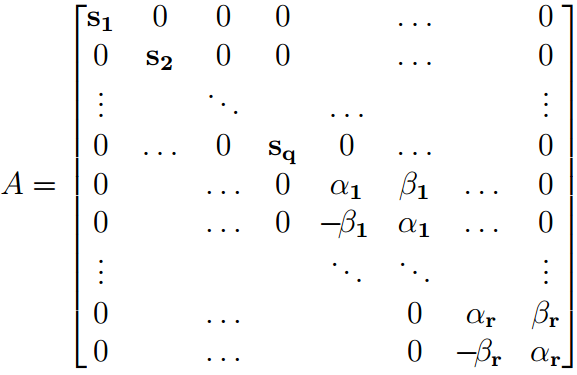
\includegraphics[scale = 0.50]{images/1.png}
		\label{image:1}
	\end{figure}
	
	В отличие от предыдущего случая мнимым корням соответствует матрица 2x2 следующего вида:
	
	\begin{figure}[h!]
		\centering
		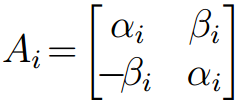
\includegraphics[scale = 0.57]{images/2.png}
		\label{image:2}
	\end{figure}
	
	\item \emph{\textbf{Кратные вещественные и комплексные корни}}
	
	Пусть имеется кратные корни: $s_1$ - кратности $l_1,s_2$ - кратности $l_2,...,s_p$ - кратности $l_p$. Выполнено условие $\sum_{i=1}^{p}l_i=n$. Тогда матрица А имеет следующую блочную структуру:
	
	\begin{figure}[h!]
		\centering
		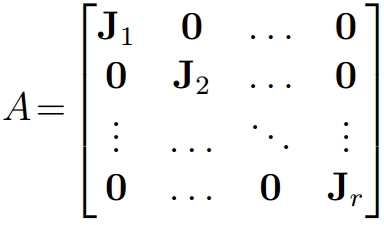
\includegraphics[scale = 0.50]{images/3.png}
		\label{image:3}
	\end{figure}
	
	Блочно-диагональная форма матрицы А называется вещественной Жордановой матрицей.
	
	$J_i, i=1,2,...,r,$ r - ящики Жордана, имеющие вид: 
	
	\begin{itemize}
		\item Для вещественных корней $Ims_j=0$:
		
		\begin{figure}[h!]
			\centering
			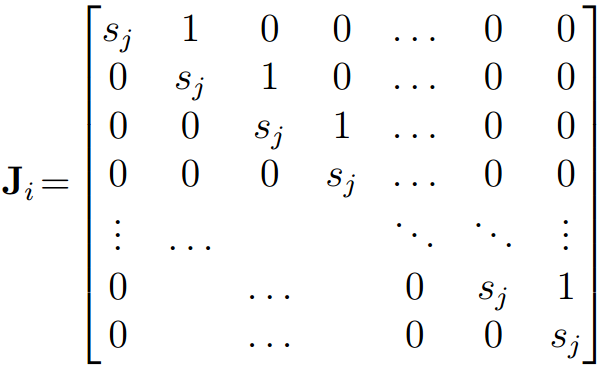
\includegraphics[scale = 0.40]{images/4.png}
			\label{image:4}
		\end{figure}
		
		\item Для мнимых собственных чисел $s_j=\alpha_j\pm j\beta_j$:
		
		\begin{figure}[h!]
			\centering
			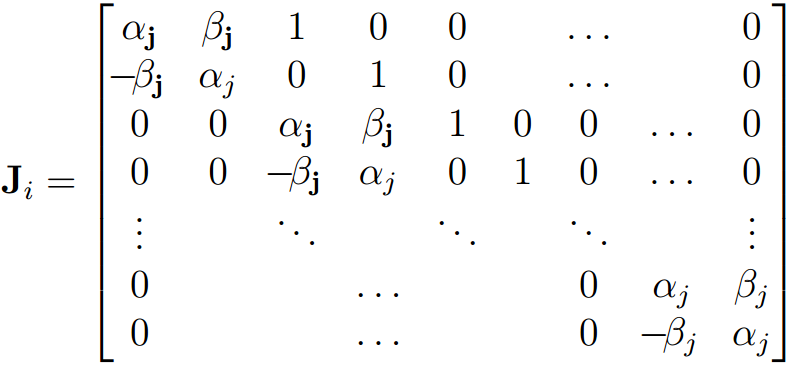
\includegraphics[scale = 0.40]{images/5.png}
			\label{image:5}
		\end{figure}
		
	\end{itemize}
		
\end{itemize}

\section{Эквивалентные преобразования форм модели ВСВ}

Обратимся теперь к задаче перехода от исходных уравнений состояния к уравнениям в заданной канонической форме. Решение этой задачи сводится к определению невырожденной n x-матрицы T такой, что для заданных матриц A, B, C получаются уравнения с матрицами $\widetilde{A}=TAT^{-1}, \widetilde{B}=TB, \widetilde{C}=CT^{-1}$, имеющими требуемый канонический вид.

\begin{itemize}
	\item \emph{\textbf{Преобразование к канонической форме}}

	\begin{itemize}
		\item \emph{Вещественные корни}
	
		Если все корни характеристического многочлена матрицы А - простые вещественные числа, тогда матрица приведения Т к диагональной канонической форме (1) определяется из выражения:
		\begin{center}
			$T=[x^0_1, x^0_2,..., x^0_n]^{-1}$
		\end{center}
		где $x^0_i(i=1,2,...,n)$ - собственные векторы матрицы А.
		
		\item \emph{Вещественные и комплексные корни}
		
		Если размер каждой клетки совпадает с кратностью соответствующего вещественного собственного значения или равен удвоенной кратности мнимых
		(комплексно-сопряженных) собственных значений, то такая матрица может быть приведена к виду Фробениуса. В противном случае такая возможность отсутствует.
		
		Рассматривая алгоритмы приведения уравнений состояния к формам НФУ и НФН, будем считать, что преобразование матрицы А к виду Фробениуса возможно.
	\end{itemize}
		
	\item \emph{\textbf{Управляемое каноническое представление}}
	
	Введем матрицы управляемости:
	\begin{center}
		$Q=[b, Ab, ..., A^{n-1}b], \widetilde{Q}=[\widetilde{b}, \widetilde{Ab}, ..., \widetilde{A}^{n-1}\widetilde{b}]$
	\end{center}
	
	Если выполнены условия $det(sI_n-A)\equiv det(sI_n-\widetilde{A}, detQ\neq0, det\widetilde{Q}\neq0)$, то существует и единственна невырожденная матрица преобразования Т, определяемая выражением	$T=\widetilde{Q}Q^{-1}$, при которой матрицы A,b и $\widetilde{A}, \widetilde{b}$ связаны соотношением $\widetilde{A}=TAT^{-1}, \widetilde{b}=Tb$.
	
	\item \emph{\textbf{Наблюдаемое каноническое представление}}
	
	Введем матрицы наблюдаемости:
	
	\begin{center}
		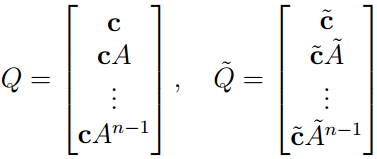
\includegraphics[width=5cm]{images/6.png}
	\end{center}
	
	При выполнении условий $det(sI_n-A)\equiv det(sI_n-\widetilde{A}, detQ\neq 0, det\widetilde{Q}\neq0$ существует и единственна невырожденная матрица преобразования $T=\widetilde{Q}^{-1}Q$ так, что матрицы A, с и $\widetilde{A}, \widetilde{c}$ связаны соотношением	$\widetilde{A}=TAT^{-1}, \widetilde{c}=cT^{-1}$.
	
	
	Всегда есть множитель $\lambda\in R, \lambda\neq0$ такой, что $x^0_i, \lambda x^0_{i+1}$ - комплексно-сопряженные. Поэтому будем считать, что выполнено условие $x^0_{i+1}=conj(x^0_i)$, где conj - операция комплексного сопряжения. Определим теперь векторы $h_i, h_{i+1}$ формулами:
	\begin{center}
		$h_i=\frac{1}{2}(x^0_i+x^0_{i+1}), h_{i+1}=\frac{1}{2\jmath}(x^0_i+x^0_{i+1})$
	\end{center}
	Векторы $h_i, h_{i+1}$ по построению вещественные и, если все собственные числа простые, линейно независимы между собой и с другими собственными векторами. Эти векторы определяют в пространстве $R^n$ некоторую собственную плоскость – инвариантное подпространство матрицы A размерности два.
	
	Построим теперь матрицу преобразования
	\begin{center}
		$T=[X^0_1, X^0_2, ..., h_j, h_{j+1}, ..., h_{q+r-1}, h_{q+r}]^{-1}$
	\end{center}
	где вектор-столбцы $x^0_i$ отвечают вещественным, а $h_j, h_{j+1}$ - мнимым собственным значениям $s_{j,j+1}=\alpha_j\pm\jmath\beta_j$.
	
	Преобразование $\widetilde{A}=TAT^{-1}$ с найденной таким образом матрицей T приводит уравнения системы к вещественной блочно-диагональной форме (1), в которой порядок следования блоков соответствует порядку расположения столбцов $x^0_i, h_j$ у матрицы $P=T^{-1}$.
	
	\begin{itemize}
		\item \emph{Кратные вещественные и комплексные корни}\\
		Из выражения $\widetilde{A}=TAT^{-1}$, следует что:
		\begin{center}
			$\widetilde{A}T=TA$
		\end{center}
		
		Обозначим столбцы матрицы Т как $q_1, q_2, ..., q_n$. Тогда из формы (3) матрицы А с учетом предыдущей формулы получим $Aq_i-\lambda q_i+\gamma_iq{i-1}$, где $\gamma_i$ принимает значение 0 или 1 в зависимости от А, а $\lambda$ - характеристическое число матрицы А.
		
		Пусть разбиение блока $T_i$ матрицы T, соответствующее разбиению блока $J_i$ - в форме (4) или (5) в зависимости от вида корня - имеет вид $T_{i1}, T_{i2}, ..., T_{il_i}$. Тогда число $\gamma_i$ равно нулю, когда соответствующий столбец $q_i$ матрицы Т является первым столбцом подблока. Так как, при $\gamma_i$ вектор $q_i$ является собственным вектором матрицы А, можно найти первые столбцы каждого подблока как собственные векторы матрицы А. Оставшиеся столбцы каждого подблока тогда получаются из (*) при $\gamma_i=1$. Такие оставшиеся столбцы известны как обобщенные собственные векторы. Этот процесс останавливается, когда $Aq_i-\lambda q_i+\gamma_iq{i-1}$ обеспечивает получение решения.
	\end{itemize}
		
\end{itemize}






\end{document}